%% Should be included with the command: \includestandalone[width=.30\textwidth]{tikz-diagrams/diagram}
%% Folder = tikz-diagrams ; file = tikz-diagrams/diagram.tex

\documentclass[crop,tikz,12pt]{standalone}


% +-----------------------------------------------------+
% |            +-- Acquisition à chaud --+              |
% |            v                         v              |
% +-------------------------+---------------------------+
% | Isolé du réseau (USB)   | Via le réseau             |
% +-----------------------------------------------------+
% | Acquisition en bootant sur un autre OS              |
% +-----------------------------------------------------+
% | Acquisition à froid (extraction du disque et copie) |
% +-----------------------------------------------------+


\begin{document}
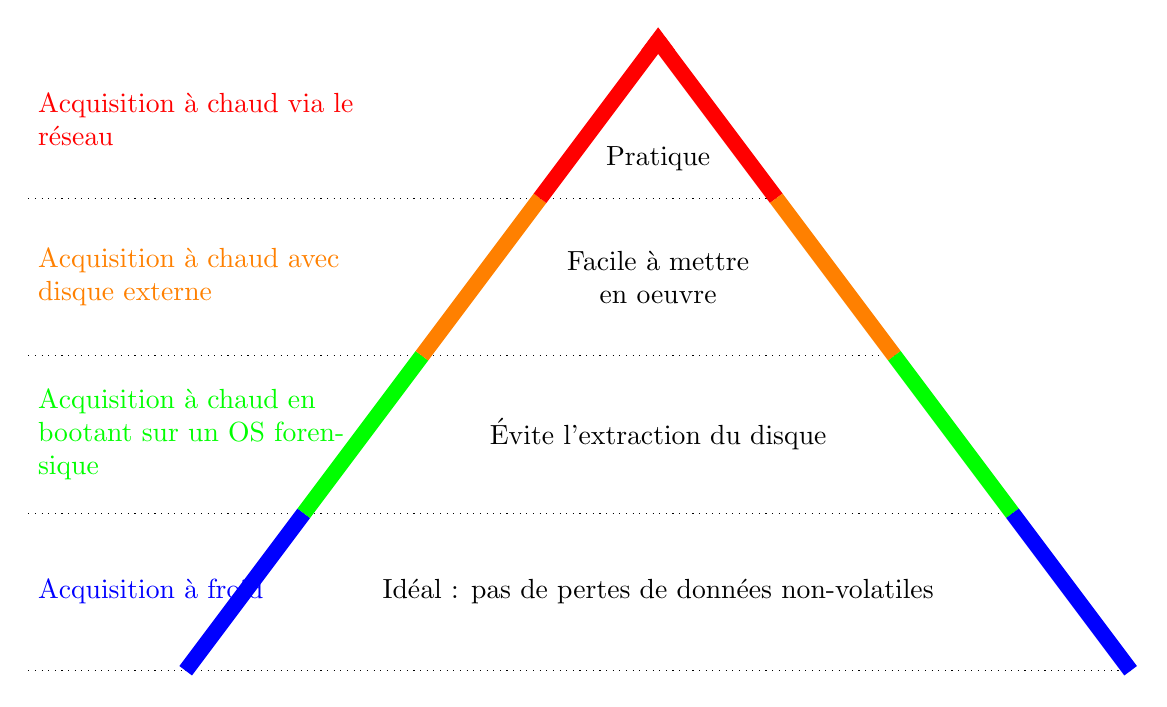
\begin{tikzpicture}

    \draw (0,0) -- (6,8);
    \draw (12,0) -- (6,8);

    \foreach \i in {0,...,3} {
        \draw[dotted] (-2, 2*\i) -- (12-1.5*\i, 2*\i);
    }

    \draw[blue,line width=0.2cm]   (0.0,0) -- (1.5,2);
    \draw[green,line width=0.2cm]  (1.5,2) -- (3.0,4);
    \draw[orange,line width=0.2cm] (3.0,4) -- (4.5,6);
    \draw[red,line width=0.2cm]    (4.5,6) -- (6.0,8);

    \draw[red,line width=0.2cm]    (6.0,8) -- (7.5,6);
    \draw[orange,line width=0.2cm] (7.5,6) -- (9.0,4);
    \draw[green,line width=0.2cm]  (9.0,4) -- (10.5,2);
    \draw[blue,line width=0.2cm]   (10.5,2) -- (12.0,0);

    \draw[red,fill=red] (6,8.16) -- (5.8,7.89) -- (6.2,7.89) -- cycle;

    \node () [red,anchor=west,text width=4.5cm]    at (-2,7) {Acquisition à chaud via le réseau};
    \node () [orange,anchor=west,text width=4.5cm] at (-2,5) {Acquisition à chaud avec disque externe};
    \node () [green,anchor=west,text width=4.2cm]  at (-2,3) {Acquisition à chaud en \\ bootant sur un OS forensique};
    \node () [blue,anchor=west,text width=3cm]     at (-2,1) {Acquisition à froid};

    \node () [] at (6,1.0) {Idéal : pas de pertes de données non-volatiles};
    \node () [] at (6,3.0) {Évite l'extraction du disque};
    \node () [text width=3cm, text centered] at (6,5.0) {Facile à mettre \\ en oeuvre};
    \node () [] at (6,6.5) {Pratique};

\end{tikzpicture}
\end{document}
